\documentclass[12pt,a4paper]{article}
\usepackage[T1]{fontenc} 
\usepackage[a4paper]{geometry}
\usepackage[brazil]{babel}
\usepackage[utf8]{inputenc}
\usepackage{setspace}
\usepackage{libertine}
 
\usepackage{url}

\usepackage{hyperref}

\usepackage{cite}  % Needed to use citations.

\usepackage{color,graphicx}
\usepackage{xcolor} 
 
\title{Visualizador de Protótipos com Realidade Virtual}
%\author{Humberto Lino Dias \\  \href{mailto:hldtux@gmail.com}{hldtux@gmail.com} }
%\author{Humberto Lino Dias \\ hldtux@gmail.com}
\author{Humberto Lino Dias}

 
\begin{document}
\maketitle

\abstract{O artigo apresenta um trabalho realizado na área de prototipação virtual. É descrito um
procedimento para a implementação de um protótipo de um torno CNC utilizando um software para
desenvolvimento em ambientes virtuais. Este procedimento enfoca principalmente o sistema de
intertravamento (funcionalidade) e modelo geométrico (design físico) do torno. Consequentemente
este trabalho visa verificar as potencialidades e as limitações desta ferramenta de interação gráfica
diante da complexidade dos dados que a prototipação de um produto de manufatura ou montagem
requer.}

\pagenumbering{gobble}
\singlespacing
 
 
\section{Óculos para Realidade Virtual}

\begin{center}

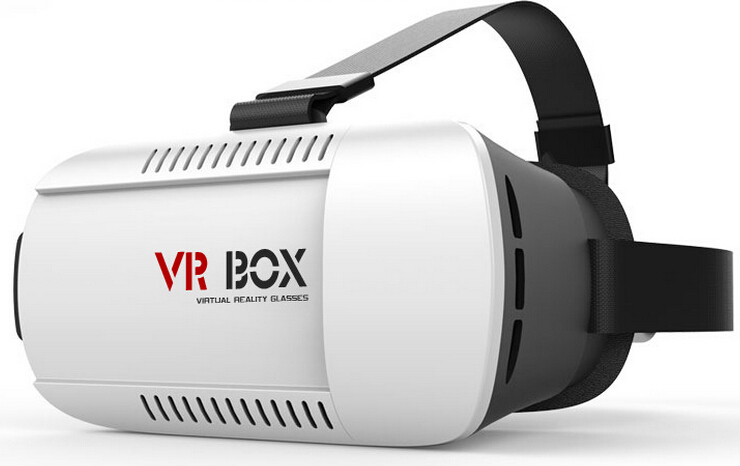
\includegraphics[height=3.1in]{vr-box-head-set.eps} \\ [1em]
\textbf{HeadSet}: VR-Box, Óculos de realidade virtual.\cite{vr_vbox_head_set}

\end{center}

 
\subsection{INTRODUÇÃO}

\paragraph{}
Prototipação virtual é um passo importante em direção
ao desenvolvimento eficiente do produto final.
Baseados nas informações de geometria e topologia do
projeto, nos resultados da simulação obtidos por
ferramentas de modelagem combinados com os cálculos
de cinemática, o material, a tolerância e outras
informações disponíveis sobre o produto, será possível
gerar protótipos no computador para apresentações
realistas, diminuindo os custos com protótipos reais e
com o tempo de disponibilização para testes, permitindo
ainda interações com o produto até mesmo nos estágios
iniciais de desenvolvimento (Rix et al., 1995).

\paragraph{}
Pode-se utilizar a realidade virtual para desenvolver e testar um Sistema de
Intertravamento de maneira rápida para atender às necessidades deste novo mercado. A
realidade virtual é uma avançada interface homem-computador que simula um ambiente real e
permite aos participantes interagirem com o mesmo (Valério Netto, 1997). Assim com o uso da
simulação de um Sistema de Intertravamento em ambiente de realidade virtual, cria-se um
protótipo virtual de um sistema, reduzindo-se os custos e o tempo de desenvolvimento deste
Sistema, uma vez que são eliminados etapas de confecção de protótipos físicos, bem como
proporciona-se uma melhoria da qualidade do produto, pois a aplicação de diferentes
alternativas do projeto pode ser realizada mais rapidamente, permitindo uma melhoria da
validação das soluções apropriadas que satisfaça os parâmetros especificados para o sistema,
com um menor custo. Segundo Kinner ( 1996 ):

\subsection{VISÃO GERAL DO PROJETO PRÁTICO}
\paragraph{}
Nesta fase, toda a comunicação era feita apenas pela fala, o que tornava o \hyphenation{co-nhe-ci-men-to} restrito aos grupos que se comunicavam com a mesmo dialeto. Além de ser uma comunicação de meio ruidoso. Ou seja, quanto mais a mensagem trafega, mais ela se distancia da versão original. Característica que não ocorre na galáxia seguinte.

\subsection{PROCEDIMENTO PARA A IMPLEMENTAÇÃO}

\paragraph{}
É marcada pelo início da prensa de \textbf{Gutenberg}.
Com ela a cultura e o conhecimento puderam então, serem passadas adiante de forma direta.
Para Mcluhan, a imprensa é o livro diário das pessoas e ele atribui à ela o crescimento do nacionalismo. 
Mesmo não sendo ruidosa, ainda existiam barreiras linguísticas, que foram sobrepostas pela linguagens regionais da imprensa.

\subsection{CONCLUSÕES}
\paragraph{}
O avanço significativo da tecnologia permitiu que todo o conhecimento ficasse disponível e com fácil acesso.
Sendo a comunicação instantânea e a velocidade com que as informações são passadas é incrivelmente alta.
Uma crítica que Mcluhan\cite{wiki:marshall_mcluhan} faz, é que com o acesso rápido e fácil ao conhecimento, as pessoas não se esforçam tanto para memorizar como antes. \cite{ted:ted_talk_feats_of_memory_anyone_can_do}
Mcluhan também fala sobre os novos meios de comunicação.
Segundo ele, as novas mídias situam certas personalidade em um novo plano de existência.
O que cada uma dessas personalidade faz, se torna ponto de consciência coletiva para uma sociedade inteira.


 
\bibliography{refs}
\bibliographystyle{plain}
 
\end{document}